%; whizzy paragraph -pdf xpdf -latex ./whizzypdfptex.sh
%; whizzy-paragraph "^\\\\begin{frame}\\|\\\\emtext"
% latex beamer presentation.
% platex, latex-beamer $B$G%3%s%Q%$%k$9$k$3$H$rA[Dj!#(B 

%     Tokyo Debian Meeting resources
%     Copyright (C) 2012 Junichi Uekawa

%     This program is free software; you can redistribute it and/or modify
%     it under the terms of the GNU General Public License as published by
%     the Free Software Foundation; either version 2 of the License, or
%     (at your option) any later version.

%     This program is distributed in the hope that it will be useful,
%     but WITHOUT ANY WARRANTY; without even the implied warreanty of
%     MERCHANTABILITY or FITNESS FOR A PARTICULAR PURPOSE.  See the
%     GNU General Public License for more details.

%     You should have received a copy of the GNU General Public License
%     along with this program; if not, write to the Free Software
%     Foundation, Inc., 51 Franklin St, Fifth Floor, Boston, MA  02110-1301 USA

\documentclass[cjk,dvipdfmx,12pt]{beamer}
\usetheme{Tokyo}
\usepackage{monthlypresentation}

%  preview (shell-command (concat "evince " (replace-regexp-in-string "tex$" "pdf"(buffer-file-name)) "&")) 
%  presentation (shell-command (concat "xpdf -fullscreen " (replace-regexp-in-string "tex$" "pdf"(buffer-file-name)) "&"))
%  presentation (shell-command (concat "evince " (replace-regexp-in-string "tex$" "pdf"(buffer-file-name)) "&"))

%http://www.naney.org/diki/dk/hyperref.html
%$BF|K\8l(BEUC$B7O4D6-$N;~(B
\AtBeginDvi{\special{pdf:tounicode EUC-UCS2}}
%$B%7%U%H(BJIS$B7O4D6-$N;~(B
%\AtBeginDvi{\special{pdf:tounicode 90ms-RKSJ-UCS2}}

\newenvironment{commandlinesmall}%
{\VerbatimEnvironment
  \begin{Sbox}\begin{minipage}{1.0\hsize}\begin{fontsize}{8}{8} \begin{BVerbatim}}%
{\end{BVerbatim}\end{fontsize}\end{minipage}\end{Sbox}
  \setlength{\fboxsep}{8pt}
% start on a new paragraph

\vspace{6pt}% skip before
\fcolorbox{dancerdarkblue}{dancerlightblue}{\TheSbox}

\vspace{6pt}% skip after
}
%end of commandlinesmall


\title{Raspberry Pi 2 Model B $B$K(B Debian Jessie / armhf $B$r%$%s%9%H!<%k$9$k(B}
\subtitle{$BBh(B125$B2s(B 2015$BG/(B3$B7nEY(B}
\author{$B4d>>(B $B?.MN(B}
\date{2015$BG/(B3$B7n(B7$BF|(B}
\logo{
\includegraphics[width=8cm]{image200607/openlogo-light.eps}}

\begin{document}

\begin{frame}
\titlepage{}
\end{frame}

\begin{frame}{$B%"%8%'%s%@(B}
\begin{enumerate}
\item Raspberry Pi 2 Model B $B$H(B Raspberry Pi $B$N0c$$(B
\item Raspberry Pi 2 Model B $B$K(B Debian Jessie / armhf $B$r%$%s%9%H!<%k$9$k(B
\end{enumerate}
\end{frame}



\emtext{Raspberry Pi 2 Model B $B$H(B Raspberry Pi $B$N0c$$(B}

\begin{frame}{Raspberry Pi 2$B$H$O!)(B}
\begin{itemize}
\item 2015$BG/(B2$B7n(B2$BF|$KH/Gd$5$l$??7$7$$(B Raspberry Pi
\item CPU$B!"%a%b%j$N6/2=(B
\item Raspberry Pi 2 $B$G$O(B Debian armhf $B$,MxMQ$G$-$k(B
\item Raspbian $B;H$o$J$/$F$bNI$/$J$C$?!#(B
\item Raspbian is not Debian
\end{itemize}
\end{frame}

\begin{frame}{Raspberry Pi 2 Model B $B$H(B Raspberry Pi $B$N0c$$(B}
\begin{figure}[htbp]
\begin{center}
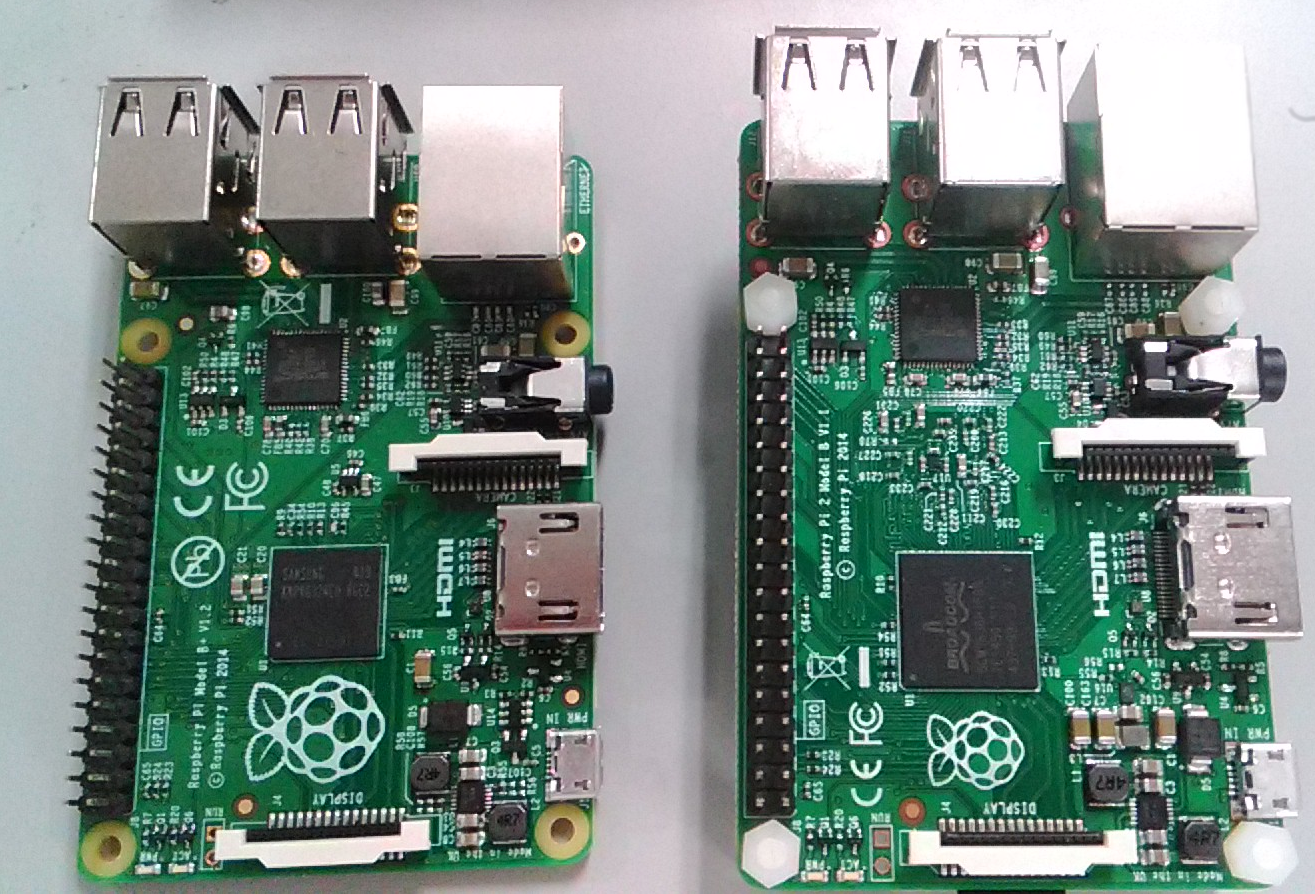
\includegraphics[width=0.7\hsize]{image201503/rpis.png}
\end{center}
\end{figure}
\end{frame}

\begin{frame}[containsverbatim]{Raspberry Pi 2 Model B $B$H(B Raspberry Pi $B$N0c$$(B}

\resizebox{\textwidth}{!}{
\begin{tabular}{|c|c|c|}
\hline
-   & RPi Model B+ & RPi 2 Model B \\
\hline
\hline
CPU  & ARM1176JZF-S 1$B%3%"(B (700MHz) / ARMv6 & {\color{red}ARM Cortex-A7 4$B%3%"(B (900MHz) / ARMv7}\\
\hline
SoC  & Broadcom BCM2835 &  Broadcom BCM2836 \\  
\hline
CPU  & Broadcom VideoCore IV (250MHz) & $BF1:8(B \\
\hline
$B%a%b%j(B & 512MB (SDRAM)& {\color{red}1GB (LPDDR2 SDRAM)} \\
\hline
$B%M%C%H%o!<%/(B & LAN9514 (10/100 Mbps) & $BF1:8(B \\
\hline
$B30It(BI/O & GPIO 40$B%T%s(B & $BF1:8(B \\
\hline
$B%9%H%l!<%8(B & microSD & $BF1:8(B \\
\hline
$BEE8;(B & 600 mA (3.0W) & {\color{red}900 mA (4.5-5.5W)} \\
\hline
\end{tabular}
}
\end{frame}

\begin{frame}{Raspberry Pi 2 Model B $B$H(B Raspberry Pi $B$N0c$$(B}

\resizebox{\textwidth}{!}{
\begin{tabular}{|c|c|c|c|}
\hline
 - & Debian armel & Debian armhf & Raspbian \\
\hline
\hline
$B%?!<%2%C%HL?Na%;%C%H(B &  ARMv4 & ARMv7 & ARMv6 \\
\hline
FPU &  $B$J$7(B &  VFPv3  &  VFPv2 \\
\hline
Debian $B%M%$%F%#%V(B & Yes & Yes & No \\
\hline
\end{tabular}
}
\end{frame}

\begin{frame}{Raspberry Pi 2 Model B $B$H(B Raspberry Pi $B$N0c$$(B}

Unixbench (System Benchmarks Index Score) 
\resizebox{\textwidth}{!}{
\begin{tabular}{|c|c|c|c|}
\hline
Debian armel / RPi & Debian armhf /RPi2 & Raspbian / Rpi & Raspbian / Rpi2 \\
\hline
66.5 & 450.8 (128.9) & 80.1 & 442.99\\
\hline
\end{tabular}
}
\end{frame}

\emtext{Debian armhf / Jessie $B$N%$%s%9%H!<%kJ}K!(B}

\begin{frame}{Debian armhf / Jessie $B$N%$%s%9%H!<%kJ}K!(B}

$B=`Hw$9$k$b$N(B

\begin{itemize}
\item $B<B5!(B
\item $B=i4|2=$5$l$F$b$h$$(B4GB$B0J>e$N(BmicroSD$B%+!<%I(B
\item $BEE8;MQ$N(Bmicro USB $B%1!<%V%k(B
\item USB$B%7%j%"%kJQ49%b%8%e!<%k(B
\end{itemize}

\end{frame}

\begin{frame}{$B@\B3Nc(B}
\begin{figure}[htbp]
\begin{center}
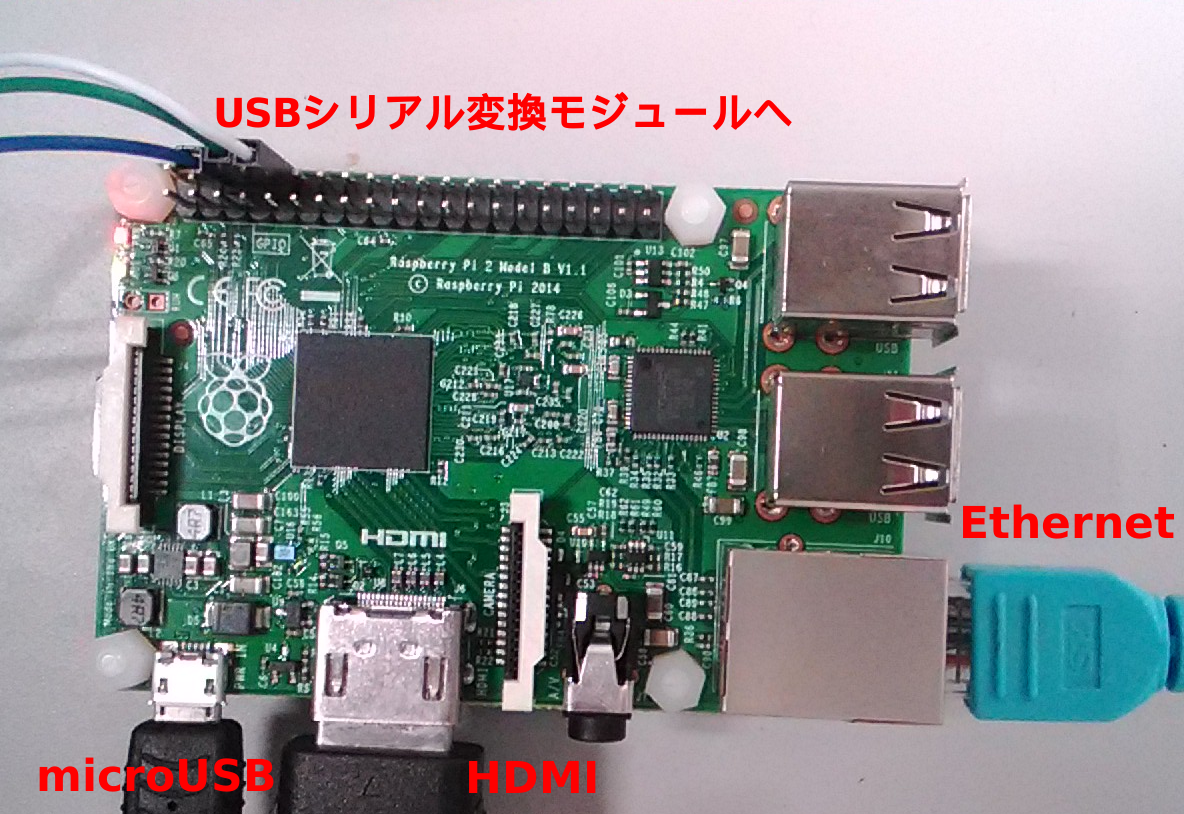
\includegraphics[width=0.7\hsize]{image201503/rpi2-hw-setting.png}
\end{center}
\caption{RPi2 $B@\B3Nc(B}
\label{fig:rpi2-hw-setting}
\end{figure}
\end{frame}

\begin{frame}{$B:n6H$NN.$l(B}
\begin{enumerate}
\item microSD$B%+!<%I$NG'<13NG'(B
\item microSD$B%+!<%I$N=i4|2=(B
\item microSD$B%+!<%I$K%Q!<%F%#%7%g%s:n@.(B
\item microSD$B%+!<%I$N%U%)!<%^%C%H(B
\item cdebootstrap $B$r;H$C$F(BmicroSD$B%+!<%I$K%$%s%9%H!<%k(B
\item RPi2$B$N(BLinux$B%+!<%M%k$H%+!<%M%k%b%8%e!<%k$N%$%s%9%H!<%k(B
\item RPi2$B$N%+!<%M%k%3%^%s%I%i%$%s$N@_Dj(B
\item fstab$B$N@_Dj(B
\item $B%M%C%H%o!<%/%G%P%$%9$N@_Dj(B
\item rootfs$BMQ%Q!<%F%#%7%g%s$NJQ99(B
\item root $B$N%Q%9%o!<%I$N@_Dj$H(Brpi$B%f!<%6$NDI2C(B
\item microSD$B%+!<%I$N%"%s%^%&%s%H$H(BRPi2$B$N5/F0(B
\item RPi2 $B$X$N%m%0%$%s(B
\item RPi2 $B@lMQ%D!<%k$N%$%s%9%H!<%k(B
\end{enumerate}
\end{frame}

\begin{frame}[containsverbatim]{microSD$B%+!<%I$NG'<13NG'(B}

\begin{commandline}
$ dmesg  | tail -5
[858983.896718] FAT-fs (sdf1): Directory bread(block 32775) failed
[858983.896729] FAT-fs (sdf1): Directory bread(block 1390704) failed
[858983.896731] FAT-fs (sdf1): Directory bread(block 1390705) failed
[869873.800361] sd 6:0:0:3: [sde] 15523840 512-byte logical blocks: (7.94 GB/7.40 GiB)
[869873.831121]  sde: sde1
\end{commandline}

\end{frame}

\begin{frame}[containsverbatim]{microSD$B%+!<%I$N=i4|2=(B}

\begin{commandline}
$ sudo dd if=/dev/zero of=/dev/sde bs=1M count=1
\end{commandline}

\end{frame}

\begin{frame}[containsverbatim]{microSD$B%+!<%I$K%Q!<%F%#%7%g%s:n@.(B}

\begin{commandline}
$ sudo fdisk /dev/sde
Command (m for help): o
...
Command (m for help): n
...
Select (default p): p
...
Partition number (1-4, default 1): 1
...
Last sector, +sectors or +size{K,M,G,T,P} \
	     (2048-15523839, default 15523839): +32M
...
Command (m for help): t
...
Hex code (type L to list all codes): e
...
Command (m for help): n
...
Select (default p): p
...
Partition number (2-4, default 2): 2
...
Command (m for help): w
\end{commandline}

\end{frame}

\begin{frame}[containsverbatim]
\begin{commandline}
(echo o; echo n; echo p; echo 1; echo ; echo +32M; \
 echo t; echo e; echo n; echo p; echo 2; echo ; echo ; \
 echo w) | fdisk /dev/sde
\end{commandline}
\end{frame}

\begin{frame}[containsverbatim]{microSD$B%+!<%I$N%U%)!<%^%C%H(B}

\begin{commandline}
$ sudo mkfs.msdos /dev/sde1
$ sudo mkfs.ext4 /dev/sde2
$ mkdir /tmp/boot /tmp/rootfs
$ sudo mount /dev/sde1 /tmp/boot
$ sudo mount /dev/sde2 /tmp/rootfs
\end{commandline}
\end{frame}

\begin{frame}[containsverbatim]{cdebootstrap $B$r;H$C$F(BmicroSD$B%+!<%I$K%$%s%9%H!<%k(B}

\begin{commandline}
$ sudo cdebootstrap --arch=armhf -f standard \
  --foreign jessie \
  --include=openssh-server,ntp,ca-certificates,vim \
  /tmp/rootfs
...
\end{commandline}

\end{frame}

\begin{frame}[containsverbatim]{RPi2$B$N(BLinux$B%+!<%M%k$H%+!<%M%k%b%8%e!<%k$N%$%s%9%H!<%k(B}

\begin{itemize}
\item RPi2$B$N(BLinux$B%+!<%M%k$O(BDebian$B$G$ODs6!$5$l$F$$$J$$(B
\item $B40A4$K%"%C%W%9%H%j!<%`$G%5%]!<%H$5$l$F$$$J$$(B
\item $B5/F0$K%U%!!<%`%&%'%"$,I,MW(B
\item Debian$B$G(B RPi2 $B$N(BLinux$B%+!<%M%k$r07$&$K$O(Brpi-update $B$r;H$C$F:G?7%+!<%M%k$r%3%T!<$9$k(B
\end{itemize}

\end{frame}

\begin{frame}[containsverbatim]{RPi2$B$N(BLinux$B%+!<%M%k$H%+!<%M%k%b%8%e!<%k$N%$%s%9%H!<%k(B}
\begin{commandline}
$ sudo curl -o /tmp/rootfs/usr/bin/rpi-update https://raw.githubusercontent.com/Hexxeh/rpi-update/master/rpi-update
$ sudo chmod +x /tmp/rootfs/usr/bin/rpi-update
$ sudo mkdir /tmp/rootfs/lib/modules
$ sudo ROOT_PATH=/tmp/rootfs BOOT_PATH=/tmp/boot /tmp/rootfs/usr/bin/rpi-update
*** Raspberry Pi firmware updater by Hexxeh, enhanced by AndrewS and Dom 
 *** Performing self-update
  % Total    % Received % Xferd  Average Speed   Time    Time     Time  Current
                                 Dload  Upload   Total   Spent    Left  Speed
100  8107  100  8107    0     0  54471      0 --:--:-- --:--:-- --:--:-- 54777
 *** Relaunching after update
...
\end{commandline}
\end{frame}

\begin{frame}[containsverbatim]{RPi2$B$N%+!<%M%k%3%^%s%I%i%$%s$N@_Dj(B}

\begin{commandline}
$ sudo sh -c "echo dwc_otg.lpm_enable=0 console=ttyAMA0,115200 console=tty1
     root=/dev/mmcblk0p2 rootwait > /tmp/boot/cmdline.txt
\end{commandline}
\end{frame}

\begin{frame}[containsverbatim]{fstab$B$N@_Dj(B}

\begin{commandline}
proc            /proc           proc    defaults	0	0
/dev/mmcblk0p1  /boot           vfat    defaults	0	2
/dev/mmcblk0p2  /               ext4    defaults,noatime	0	1
\end{commandline}

\end{frame}

\begin{frame}[containsverbatim]{$B%M%C%H%o!<%/%G%P%$%9$N@_Dj(B}

\begin{commandline}
auto eth0
iface eth0 inet dhcp
\end{commandline}
\end{frame}

\begin{frame}[containsverbatim]{rootfs$BMQ%Q!<%F%#%7%g%s$NJQ99(B}

\begin{commandline}
trap 'error "Interruped!"' HUP INT TERM

mount -n -o remount,rw rootfs / <- $B$3$l$r(B
mount -n -o remount,rw /dev/mmcblk0p2 / <- $B$3$l$KJQ99(B

chown -hR 0:0 /
\end{commandline}
\end{frame}

\begin{frame}[containsverbatim]{root $B$N%Q%9%o!<%I$N@_Dj$H(Brpi$B%f!<%6$NDI2C(B}
\begin{commandline}
echo 'deb http://ftp.debian.org/debian jessie main' > /etc/apt/sources.list

echo "root:root" | chpasswd <- $B$3$N9T$rDI2C(B
useradd -m rpi <- $B$3$N9T$rDI2C(B
echo rpi:rpi | chpasswd <- $B$3$N9T$rDI2C(B

run rm /sbin/init
\end{commandline}
\end{frame}

\begin{frame}[containsverbatim]{microSD$B%+!<%I$N%"%s%^%&%s%H$H(BRPi2$B$N5/F0(B}

\begin{enumerate}
\item microSD$B%+!<%I$r%"%s%^%&%s%H$7!"(BPRi2 $B$N(B microSD$B%+!<%I%9%m%C%H$KA^F~$9$k!#(B
\item $BA^F~8e!"(Bmicro USB $B%1!<%V%k$r(B RPi2 $B$KA^$7!"(BRPi2$B$r5/F0$9$k!#(B
\item $B5/F0$9$k$H<+F0E*$K(B2nd bootstrap$B$,<B9T$5$l!"(BRPi2$B>e$G%$%s%9%H!<%k$,<B9T$5$l$k(B
\item 30$BJ,$[$IBT$D(B
\item $B%$%s%9%H!<%k40N;(B
\end{enumerate}
\end{frame}

\begin{frame}[containsverbatim]{RPi2 $B$X$N%m%0%$%s(B}

\begin{itemize}
\item USB$B%7%j%"%k%b%8%e!<%k7PM3(B
\item SSH $B7PM3(B
\item HDMI $B%b%K%?!J(Btty$B!K7PM3(B
\end{itemize}

\end{frame}

\begin{frame}[containsverbatim]{RPi2 $B@lMQ%D!<%k$N%$%s%9%H!<%k(B}

\begin{itemize}
\item RPi $B$N@lMQ%D!<%k$G$"$k(B rpi-update$B!"(Braspi-config $B$O$^$@(BDebian
$B$G$ODs6!$5$l$F$$$J$$(B
\item $B$3$l$i$r(B Debian $B$GMxMQ$G$-$k$h$&$K$9$k$K$O(B raspberrypi.org $B$GDs6!$5$l$F$$$k(B $B3F%D!<%k$N(B
Debian $B%Q%C%1!<%8$r%$%s%9%H!<%k$9$kI,MW$,$"$k!#(B
\end{itemize}

\end{frame}

\begin{frame}[containsverbatim]{RPi2 $B@lMQ%D!<%k$N%$%s%9%H!<%k(B}

\begin{commandline}
# wget -O - http://archive.raspberrypi.org/debian/raspberrypi.gpg.key | apt-key add - 
# echo deb http://archive.raspberrypi.org/debian wheezy main >> /etc/apt/sources.list
# apt-get update
# apt-get install rpi-update raspi-config
\end{commandline}
\end{frame}

\begin{frame}{$B=*$o$j$K(B}

\begin{itemize}
\item RPi2 $B$+$i(B $B%M%$%F%#%V$N(BDebian$B$,MxMQ$G$-$k$h$&$K$J$C$?(B
\item $B%$%s%9%H!<%i$d(BmicroSD$B%+!<%I%$%a!<%8$,=`Hw$5$l$F$$$J$/$F$b!"(Bcdebootstrap 
$B;H$($P4JC1$K%$%s%9%H!<%k$G$-$k(B
\item Raspbian is not Debian$B!#(BRPi2 $B$G$O(BDebian$B$r;H$$$^$7$g$&!#(B
\end{itemize}

\end{frame}

\end{document}

;;; Local Variables: ***
;;; outline-regexp: "\\([ 	]*\\\\\\(documentstyle\\|documentclass\\|emtext\\|section\\|begin{frame}\\)\\*?[ 	]*[[{]\\|[]+\\)" ***
;;; End: ***
